% This is "sig-alternate.tex" V2.1 April 2013
% This file should be compiled with V2.5 of "sig-alternate.cls" May 2012
%
% This example file demonstrates the use of the 'sig-alternate.cls'
% V2.5 LaTeX2e document class file. It is for those submitting
% articles to ACM Conference Proceedings WHO DO NOT WISH TO
% STRICTLY ADHERE TO THE SIGS (PUBS-BOARD-ENDORSED) STYLE.
% The 'sig-alternate.cls' file will produce a similar-looking,
% albeit, 'tighter' paper resulting in, invariably, fewer pages.
%
% ----------------------------------------------------------------------------------------------------------------
% This .tex file (and associated .cls V2.5) produces:
%       1) The Permission Statement
%       2) The Conference (location) Info information
%       3) The Copyright Line with ACM data
%       4) NO page numbers
%
% as against the acm_proc_article-sp.cls file which
% DOES NOT produce 1) thru' 3) above.
%
% Using 'sig-alternate.cls' you have control, however, from within
% the source .tex file, over both the CopyrightYear
% (defaulted to 200X) and the ACM Copyright Data
% (defaulted to X-XXXXX-XX-X/XX/XX).
% e.g.
% \CopyrightYear{2007} will cause 2007 to appear in the copyright line.
% \crdata{0-12345-67-8/90/12} will cause 0-12345-67-8/90/12 to appear in the copyright line.
%
% ---------------------------------------------------------------------------------------------------------------
% This .tex source is an example which *does* use
% the .bib file (from which the .bbl file % is produced).
% REMEMBER HOWEVER: After having produced the .bbl file,
% and prior to final submission, you *NEED* to 'insert'
% your .bbl file into your source .tex file so as to provide
% ONE 'self-contained' source file.
%
% ================= IF YOU HAVE QUESTIONS =======================
% Questions regarding the SIGS styles, SIGS policies and
% procedures, Conferences etc. should be sent to
% Adrienne Griscti (griscti@acm.org)
%
% Technical questions _only_ to
% Gerald Murray (murray@hq.acm.org)
% ===============================================================
%
% For tracking purposes - this is V2.0 - May 2012

\documentclass{sig-alternate-05-2015}
\usepackage{amsmath}
%\usepackage{algorithm}
\usepackage{algorithm2e}
\usepackage[noend]{algpseudocode}
\usepackage{eurosym}

\begin{document}


% Copyright
%setcopyright{acmcopyright}
%\setcopyright{acmlicensed}
\setcopyright{rightsretained}
%\setcopyright{usgov}
%\setcopyright{usgovmixed}
%\setcopyright{cagov}
%\setcopyright{cagovmixed}


\title{{Using Machine Learning to Set Exchange Rates for Medium Term Contracts}
}
\numberofauthors{2} 
\author{
\alignauthor
Eduardo Lori\'{e}\\
       \affaddr{Georgia Institute of Technology}\\
       \email{edlorie@gatech.edu}
\alignauthor 
Matthew Robinson \\
       \affaddr{Georgia Institute of Technology}\\
       \email{mrobinson72@gatech.edu}
}

\date{31 March 2016}

\maketitle

\section{Abstract}
This paper is focused in analyzing financial variables and machine learning methods to investigate exchange rate forecasting. Financial data is analyzed for five of the biggest US trading partners. This data is tested for its stationarity, analyzed to extract principal components, and it's correlations are investigated as well. Both linear and tree based models are tested using different variations of lag variables to better understand the impact of lags on financial data. These models are compared to the standard used random walk method. Finally an explanation is provided on why some of these methods do or do not outperform the random walk. The hopes of this work is to enable readers how to make good choices when building prediction models for exchange rates.

\section{Introduction}
International business involves considerable risk. This is especially true for manufacturers, who often make production decisions well in advance of delivery dates. Consider the position of an airline that is preparing to expand its fleet. This airline might place an order for a passenger jet that will not be completed for a year or more, with payment due upon delivery of the jet. If the buyer is American and the manufacturer is also American, this is not a problem. All of the manufacturer's production costs will be valued in US dollars, and the customer will pay in US dollars.
\par{} In contrast, consider the situation if the buyer is Canadian and the manufacturer is American. Since the manufacturer is American, the Canadian firm must pay for the jet in US dollars. Suppose the value of the US dollar appreciates 10\% relative to the Canadian dollar while the American firm is filling the order. Then, when the Canadian firm pays for the jet, it is 10\% more expensive in terms of Canadian dollars than when it ordered it. If the movement were in the opposite direction, the manufacturer would receive 10\% fewer US dollars for the jet than it expected when it was ordered. Clearly, both firms would be interested in predicting adverse currency movements in advance, and may be interested in writing expected future currency valuations into contracts. 
\par{} With this application in mind, we consider the following question: can we predict the exchange rate after one year for the top five US trading partners during the period of 1972-2015 using monthly macroeconomic data? The variables we will use to predict the exchange rate include the current exchange rate, interest rate, inflation rate and government bond yield for both countries, and several variables related to international trade and financial flows. The remainder of this section will provide an overview of relevant economic theory, a summary of past statistical research on exchange rates and an overview of the data set. In the following section, we perform exploratory data analysis to develop a basic understanding of the behavior of the time series and discern which variables are useful as predictors. Next, we develop several models for predicting exchange rates and compare their effectiveness. This paper considers both linear models and tree based approaches. In developing statistical models, the primary focus is on incorporating time series techniques and variable selection. In the conclusion, we determine that linear regression with lagged variables is the most effective method for predicting exchange rates, evaluate the impact of this result on business decisions and suggest possible directions for future research.

\subsection{Related Work}
Equilibrium in foreign exchange markets is a well developed component of classical economic theory. Classical models rest on two fundamental ideas. The first is that foreign exchange markets achieve equilibrium when the rate of return on deposits is the same across all currencies. The idea that investors will be indifferent between bank deposits denominated in different currencies is known as interest rate parity. The second is that the price of goods will be the same when valued in different currencies. The notion that a basket of goods should cost the same across all currencies is known as purchasing power parity.
\par{} Both of these concepts rely on the same basic premise, which is that price differentials create arbitrage opportunities. Interest rate and purchasing power parity hold that price differentials are self-correcting because, as investors move to take advantage of arbitrage opportunities, they push the market back toward equilibrium. To demonstrate this idea, suppose that a laptop costs \$500 in the United States and the euro equivalent of \$550 in Germany. Someone in Germany could take advantage of this fact by buying cheap laptops in the US and selling them in Germany. This would create more demand for dollars, which are required to buy the laptops in the US, and push up US price levels. This trend would continue until price levels are high enough that laptops cost the same in the US as in Germany. When laptop prices are the same in both countries, the market is in equilibrium, since there is no longer an opportunity for arbitrage.
\par{} The following equations summarize interest rate and purchasing power parity, all else held equal. In these equations, $e_{t}$ represents the exchange rate at time $t$ in terms of the foreign currency, $i$ is the real interest rate and $\pi$ is the inflation rate. 
\begin{equation}
e_{t+1} = e_{t} \left( \frac{1+i_{d}}{1+i_{f}} \right)
\end{equation}
\begin{equation}
\frac{e_{t+1}-e_{t}}{e_{t}} = \frac{1+\pi_{d}}{1+\pi{f}} - 1
\end{equation}
\par{} In the literature, Obstfeld and Taylor show that arbitrage opportunities between foreign and domestic assets are near zero under floating currency regimes, which suggests that exchange rates behave as predicted by interest rate parity. Likewise, Frankel and Rose provide evidence that exchange rates converge to levels predicted by purchasing power parity in the long run. The relevant time-frame for the \emph{long run} in this context is about four years. Under shorter time horizons, purchasing power parity performs considerably less well. Likewise, difficulty in predicting the relative performance of financial assets in different countries makes it difficult to predict exchange rates using interest rate parity. In fact, Meese and Rogoff famously demonstrated that a random walk, which predicts no change in the exchange rate, outperforms structural models for the exchange rate over a one to twelve month window. For this reason, the random walk is currently used as a benchmark for assessing the quality of models for predicting exchange rates.
\par{} Statisticians have developed several approaches for predicting exchange rates. A model proposed by Hsiech suggests that there is little linear dependence in exchange rate movements, but strong nonlinear dependence. On the other hand, Meese and Rose showed that nonlinear estimators to do not significantly improve popular models for predicting exchange rates, and that these models do not outperform a random walk. All of these models incorporate macroeconomic variables, such as interest rates and inflation rates. Lyons and Evans produced more accurate models by incorporating microeconomic variables. They augmented previously used linear models with a new variable, order flow, which is the net of buyer and seller initiated orders. This model accurately predicted 60\% of daily changes in the exchange rate between the German Mark and the US dollar. Some researchers have also modeled exchange rates using more sophisticated machine learning techniques. Panda and Narasimhan showed that neural networks outperform both a random walk and linear autoregressive models when predicting weekly changes in the Indian rupee/US dollar exchange rate.
\par{} Past statistical research on exchange rates has largely focused on financial applications. Predicting daily or weekly exchange rate movements primarily benefits financial institutions that participate in foreign exchange markets. The goal of these firms is to profit by placing bets on currency movements. By contrast, this paper considers the problem from the perspective of an importer or exporter. Their goal is to predict medium term currency movements in order to accurately predict future costs and revenues. This helps them make more informed business decisions. Considering the medium run time horizon and using monthly data makes the problem more feasible from an economic perspective. It also makes the application less ripe for more complicated prediction techniques, such as neural networks, because the number of observations and feature space are both small. Due to these considerations, this paper will focus primarily on traditional time series techniques and variable selection.

\subsection{Data}
This paper restricts its attention to changes in the exchange rate between the United States and its five biggest trading partners, excluding China. These trading partners are Europe, Canada, Mexico, Japan and South Korea. Europe in this context refers to the 19 countries that belong to the eurozone. Since they share a common monetary policy, they will be treated as a single unit for the purposes of this paper. China is excluded because it fixes its exchange rate. Because of this, its exchange rate is determined by government policy rather than economic variables. The observations for all countries end in December 2015. The start date for the time series is 1972 for Japan, 1985 for Korea, 1990 for Canada, 1994 for Mexico and 2000 for the Euro. Japan begins in 1972 because that date marks the end of the gold standard and the beginning of the modern era of free floating currencies. For each other country, the start date was chosen as the earliest date for which data on all of the macroeconomic predictors was available. 
\par{} The data used in this paper was collected entirely by central banks and compiled by Quandl, an economic data repository. The primary variables of interest in the data set are the exchange rate, inflation rate, interest rate and the yield on one year government bonds. These are the variables that appear in the interest rate and purchasing power parity models. All exchange rates are valued as the amount of foreign currency needed to trade for one US dollar. The inflation rate measures the annualized percent change in the consumer price index for each country. The interest rate is the interbank lending rate set by the central bank for the currency in question. For the United States, this is the federal funds rate.  Other variables in the data set include an area's balance of trade, current account, foreign exchange reserves and other factors related to international financial flows. These variables were measured both for the United States and each trading partner. Each variable is measured monthly, with the exception of GDP growth, current account balance and foreign direct investment. These variables are measured quarterly. In order to align these variables with the rest of the data set, values for the intervening two months between each quarter were interpolated using cubic splines.

\section{Exploratory Data Analysis}

Before developing models to predict the exchange rate, we will begin with some preliminary exploration of the data. This section deals with two primary concerns: assessing the behavior of the time series and discerning which variables are important as predictors for the exchange rate. First, we will test whether or not the time series is stationary, then determine the degree of autocorrelation. After this, we explore basic relationships between the predictors and the exchange rate.

\subsection{Stationarity}

\begin{figure}
\centering
\caption{Stationarity in Exchange Rates}
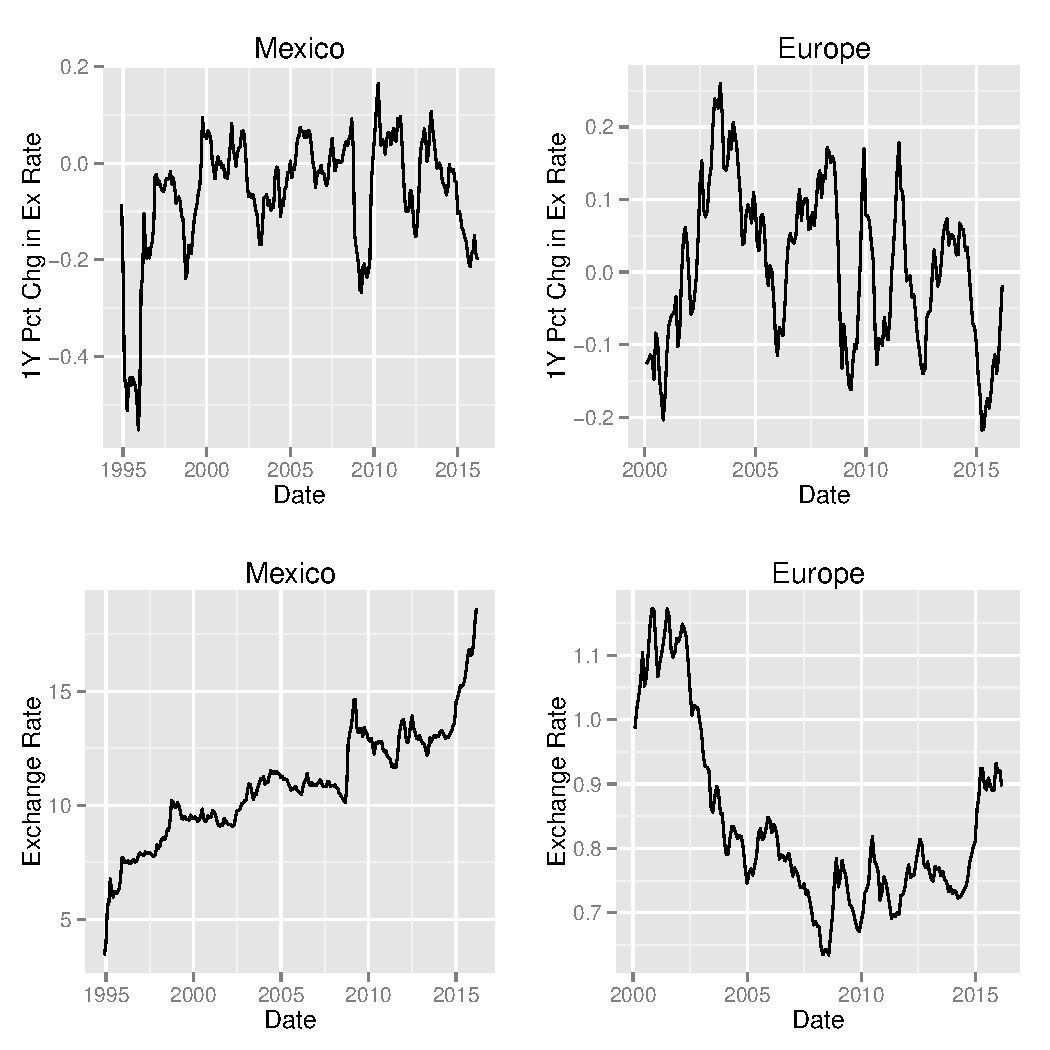
\includegraphics[scale=0.45]{stationarity.pdf}
\label{fig:rates_time}
\end{figure}

When working with a time series, it is important to consider the behavior of the stochastic process that generated the data. One important step in preliminary data analysis is determining if the stochastic process is stationary. A stochastic process is stationary if its joint probability distribution remains the same over time. This implies that the mean and variance of the stochastic process does not change.
\par{} Determining whether or not the process is stationary is important for two reasons. The first is that, if the process is not stationary, then the model must account for drift and use an estimation technique that is robust to non-constant variance. This adds complexity to the model, and makes inference more difficult. The second is that model evaluation is easier for stationary processes. In particular, realizations of a stationary process are independent of time after accounting for autocorrelation. This means that observations can be used to train a model that is validated on observations that occurred in the past without violating independence assumptions. We explore an evaluation method that takes advantage of this property below. From this, it is clear that we would prefer a stationary process, for reasons of both model complexity and ease of evaluation.
\par{} Figure ~\ref{fig:rates_time} shows the movement of both the exchange rate and the one year percent change in the exchange rate over time for both Europe and Mexico. For both countries, the exchange rates clearly drift over time. The value of the Mexican peso depreciates against the dollar over time, whereas the euro appreciates until 2008, and then begins to depreciate. Such trends imply that the exchange rate is generated by a non-stationary process. By contrast the one year percent change in the exchange rate fluctuates around a mean value for both countries, meaning the transformed process is likely stationary. Note that the two major aberrations in the graph for Mexico correspond to major exogenous financial shocks. In 1994, the Mexican government stopped pegging its exchange rate to the dollar and allowed the exchange rate to float, causing an abrupt devaluation. Likewise, the 2008 recession dramatically reduced US imports from Mexico, causing another sharp devaluation. Outside of these two periods, the behavior of the one year percent change in the value of the peso is consistent with a stationary process.
\par{} An augmented Dickey-Fuller Test was used to test the null hypothesis that that each process is non-stationary. The results appear in Figure~\ref{fig:adf}. The test statistics show that we can reject the null hypothesis that the process is non-stationary for the one year percent change time series, but fail to reject the null hypothesis for the exchange rate time series. These tests support the conclusion that the one year percent change time series is stationary, and that the exchange rate time series is non-stationary. The same results hold for Canada, Japan and Korea.
\begin{figure}
\centering
\caption{Augmented Dickey-Fuller Test}
\begin{tabular}{l l l l}
Country & Series & ADF Statistic & p-value \\
Canada & Ex. Rate & -0.965 & 0.942 \\
Canada & Pct. Change & -3.604 & 0.034  \\
Mexico & Ex. Rate & -1.796 & 0.662 \\
Mexico & Pct. Change & -3.615 & 0.032 \\
\end{tabular}
\label{fig:adf}
\end{figure}



\subsection{Autocorrelation}

\begin{figure}
\centering
\caption{Severity of Autocorrelation}
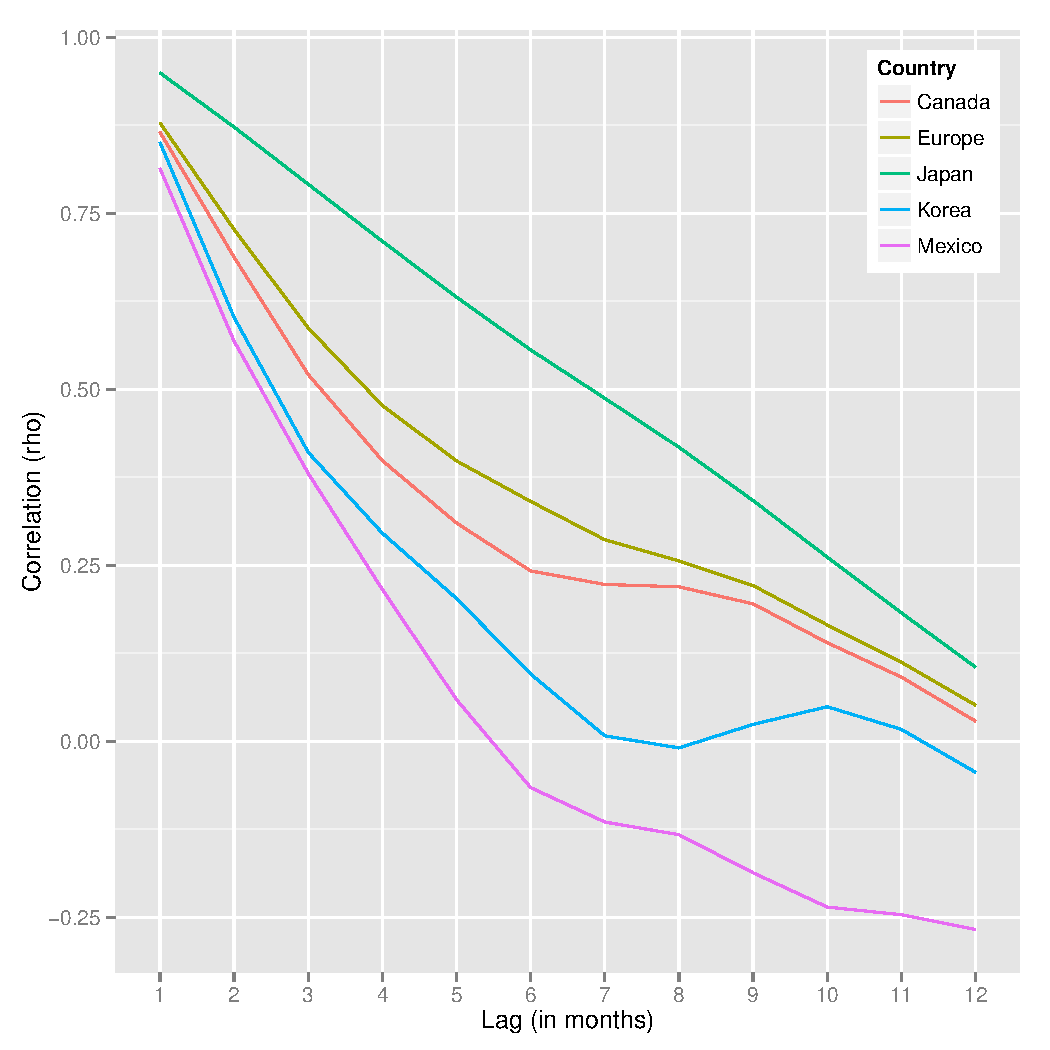
\includegraphics[scale=0.45]{autocorrelation.pdf}
\label{fig:autocorrelation}
\end{figure}

Another common feature of time series data is autocorrelation. Autocorrelation refers to correlation between values of a variable at different points in time. In order to assess the degree of autocorrelation in the exchange rate data set, we fit a simplified linear model that consisted of the current exchange rate, along with the interest rate, inflation rate and government bond yield for both countries. After fitting the model, we computed the Durbin-Watson test statistic with one to twelve month lags. Figure~\ref{fig:autocorrelation} depicts the value of the correlation coefficient for each country as a function of time.
\par{} The test statistics show that the data set exhibits strong autocorrelation for several months, and that the severity of the autocorrelation decays over time. For each country, the correlation coefficient for a one month lag is in excess of 0.80, and is as high as 0.95 for Japan. This value drops below 0.50 for every country by month four, with the exception of Japan. The persistence of autocorrelation in the case of Japan may be due to its active currency manipulation policy. For each country, the correlation coefficient remains statistically significant for at least five months. The presence of autocorrelation in the data set argues for including lagged variables in the model, through at least several months. Note that a typical lagged model includes the dependent variable at previous time steps as an independent variable. In this case, the dependent variable at time $t$ is the one year percent change in the exchange rate from one month prior, which is not known until $t+11$. For this reason, we cannot use it a predictor at time $t$. As a result, instead of lagged values of the dependent variable, we will use lagged values for each of the independent variables. For long lags, this results in a large number of possible predictors, which is why variable selection is particularly important in this problem.

%\begin{figure}
%\centering
%\caption{Durbin-Watson Test -- Canada}
%\begin{tabular}{c c c c}
%Lag & Autocorrelation & D-W Statistic & p-value \\
%1 & 0.8421 & 0.2975 & 0.000 \\
%2 & 0.6337 & 0.6994 & 0.000 \\
%3 & 0.4381 & 1.0782 & 0.000 \\
%4 & 0.2848 & 1.3816 & 0.000 \\
%5 & 0.1718 & 1.6064 & 0.014 \\
%6 & 0.0814 & 1.7851 & 0.254 \\
%\end{tabular}
%\end{figure}

%\begin{figure}
%\centering
%\caption{Durbin-Watson Test -- Japan}
%\begin{tabular}{c c c c}
%Lag & Autocorrelation & D-W Statistic & p-value \\
%1 & 0.9314 & 0.1370 & 0.000 \\
%2 & 0.8477 & 0.3041 & 0.000 \\
%3 & 0.7660 & 0.4671 & 0.000 \\
%4 & 0.6799 & 0.6388 & 0.000 \\
%5 & 0.5959 & 0.8048 & 0.000 \\
%6 & 0.5164 & 0.9615 & 0.000 \\
%\end{tabular}
%\end{figure}

\subsection{Variables}

\begin{figure}
\centering
\caption{Balance of Trade and Foreign Exchange Reserves Over Time for Japan}
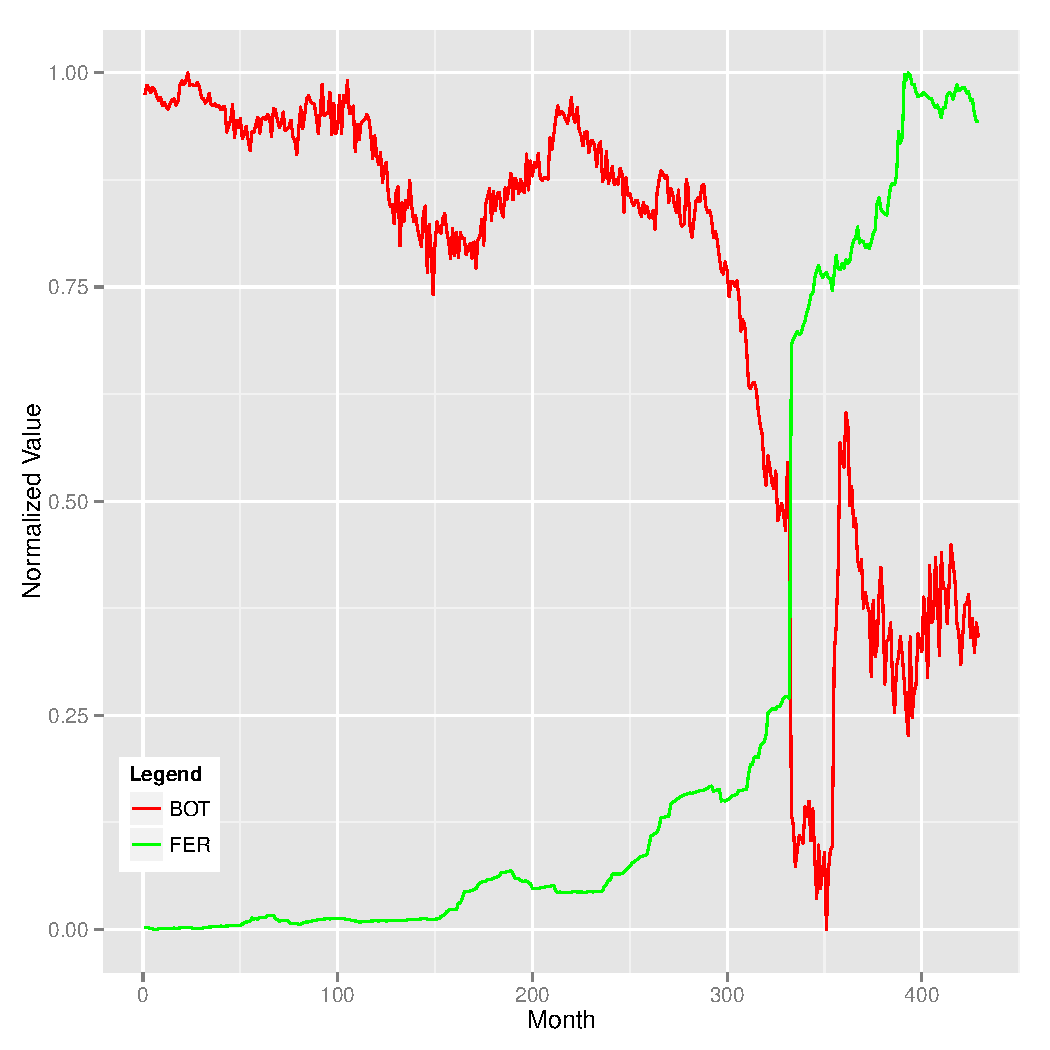
\includegraphics[scale=0.45]{japan_plot.pdf}
\label{fig:japan}
\end{figure}

\begin{figure}
\centering
\caption{Standard Deviation of Distribution for Top Ten Components}
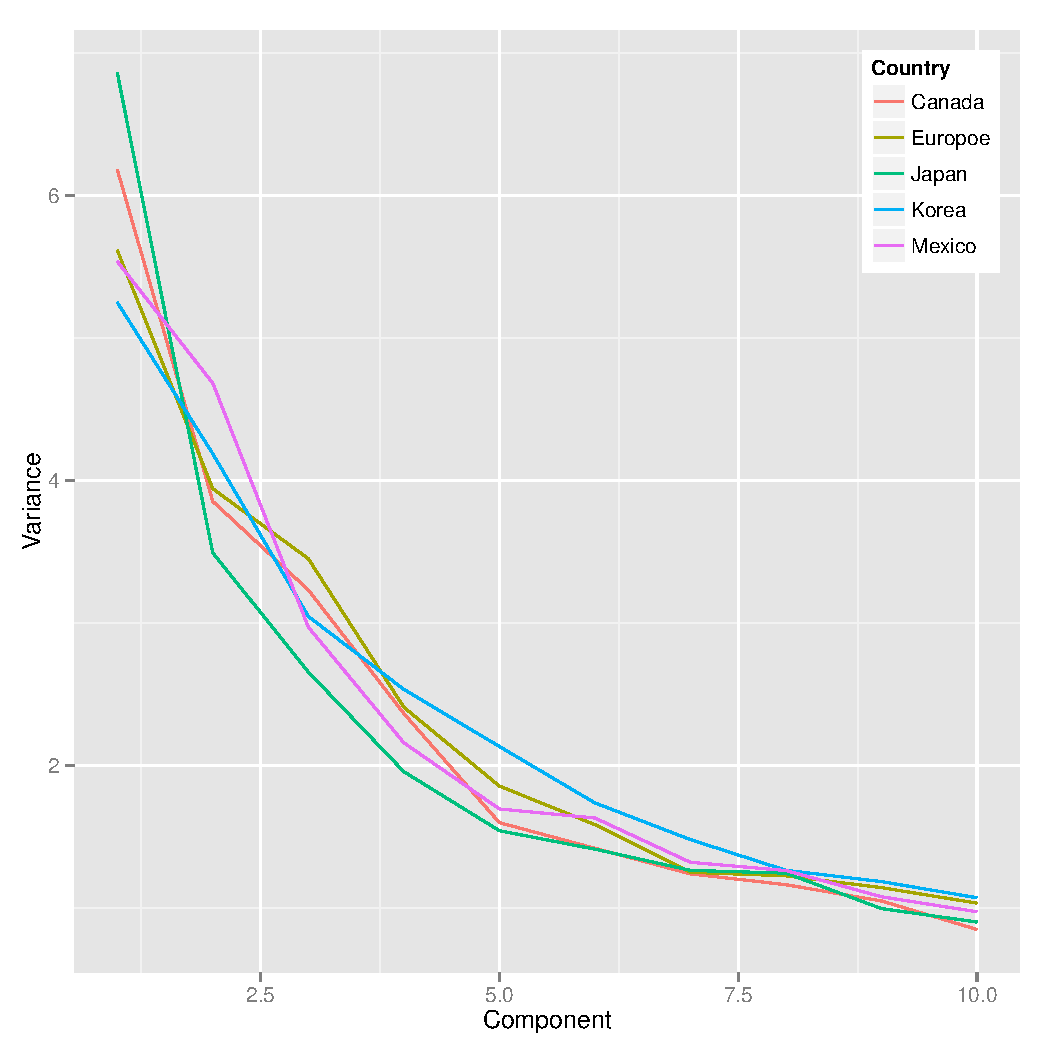
\includegraphics[scale=0.45]{prinComps.pdf}
\label{fig:japan}
\end{figure}

In order to determine basic relationships between the variables in the data set, we computed the correlation between each pair of possible predictors. The correlations that we computed were consistent with what would be expected based on the economic theory explained above. We observed high correlation between foreign and domestic interest rates and inflation rates for multiple trading partners. These results are consistent with interest rate and purchasing power parity. One noteworthy result was the high correlation between the balance of trade and foreign exchange reserves for Japan, which was 0.9. These two variables are plotted over time in Figure~\ref{fig:japan}. This makes sense, since a high balance of trade puts upward pressure on the Yen-Dollar exchange rate, and Japan sells off foreign exchange reserves in order to force down the exchange rate. Similar patterns were observed for other countries, with most of the correlations between 0.6 and 0.8. Higher levels of correlation indicate more active currency policy on the part of the central bank in question. These observations justify the inclusion of variables in the model that quantify international flows. Since foreign exchange markets involve substantial central bank involvement, we cannot expect to predict their values solely on the basis of the variables included in the standard interest rate and purchasing power parity models.

The high degree of correlation between the variables suggests that we may be able to construct a reasonably accurate low rank approximation to the matrix. As mentioned above, the inclusion of lagged variable results in a relative large feature space for longer lags. In order to determine the number of principal components, we performed principal component analysis on a data set for each country that included lags out to nine months, resulting in 77 predictor. For each country, the results show that the data set can be well approximated using nine principal components. As such, even though the number of possible predictors is very large, the degree of correlation between these predictors results in a reasonably low rank data set.

\section{Methods}
Exchange rate models must consider three important factors: which variables to include in the model, candidate methods for estimating the model and the criteria for evaluating each method. The variable selection process involves deciding which predictors to include in the model, as well as how many months of lagged observations to include. Candidate methods were chosen by considering several statistical techniques with properties that made them appealing for the exchange rate data set. These include both linear and tree based methods. Finally, we develop a method for evaluating that models that accounts for autocorrelation and leverages the stationarity of the time series.

\subsection{Variable Selection}
Selecting which variables to include in the model requires deciding which economic factors are relevant and for how many months prior to the current observation. To recap, the variables in the data set include the current exchange rate, interest rate, inflation rate and GDP growth rate for both countries, as well as several variables related to international financial flows. There is a strong theoretical justification for including each of these variables in the model. However, the number of potential predictors makes overfitting problematic, especially after the inclusion of lagged variables. We dealt with the problems of selecting the a good set of predictors and an appropriate lag simultaneously by applying the following procedure. We assessed the performance of different lags by comparing the performance of a linear regression model across a variety of lags. For each lag, the variables were chosen by forward stepwise variable selection, using AIC as the selection criteria. This technique produces a model that balances the trade off between training error and model complexity.

\subsection{Candidate Methods}
After selecting a suitable subset of variables to include in the model, we fit the model using several statistical techniques. Two families of models were considered: linear models and tree based methods. The advantage of the linear models is that they are simpler, but still powerful if they account for the structure of the time series properly. Tree based methods are considered as an alternative because of the high dimensional feature space. Since there are theoretical reasons to believe that each variable is important, ensemble methods that vary the input variables may provide superior results.

\par{} The linear models include standard linear regression, ridge regression, LASSO regression and principal components regression. Ridge regression and LASSO regression both include a regularization constant that gives preferences to models with smaller parameters in terms of absolute value. These models are appealing for the exchange rate data set because autocorrelation and the inclusion of lagged variables means the predictors in the model are highly correlated. Including a regularization constant helps prevent overfitting to the training data. For both of these models, the regularization constant is chosen using generalized cross validation. Principal component regression is potentially useful due to the large number of predictors in the model and the high correlation between those predictors. The forward stepwise variable selection technique described above results in models with 15-20 predictors, which is relatively complex for a data set that has on the order of hundreds of observations. Principal component regression simplifies the model by considering a low rank approximation of the data set that consists of the $k$ most important principal components. The number of components to include in the principal component regression was also chosen using cross validation. As noted above, the data set for each country can be well approximated with nine principal components when a nine month lag is used. This preliminary results suggests that principal component regression may be a suitable approach for this problem.

\par{} Three tree based methods are considered: full tree models, pruned tree models, and random forests. Regression trees are capable of capturing non-linear interactions between the predictors. Since the feature space for the exchange rate problem is highly interdependent and large relative to the size of the data set, tree based methods are a reasonable option to consider. Instead of using nonlinear regression, regression trees recursively partition the data. A separate model is fit for each partition. Tree based methods predict future outcomes by classifying new data into one of the partitions, and then applying the appropriate model. Each partition is represented by the nodes, or leaves, of the tree. 

\par{} Overfitting is a common concern with tree based methods. Pruning the tree is frequently used to help avoid overfitting. A tree is pruned by looking at the terminal nodes of the tree and determining if merging those nodes can decrease the entropy of the parent node. If so, the nodes are merged. Another way to avoid overfitting is to use random forests. Random forests take an ensemble of trees and return the average output of all the trees in the ensemble as the predicted value. This method avoids the high bias that is generally associated with full tree models.

\subsection{Model Evaluation}
Evaluating the effectiveness of each model requires splitting the data into training and test sets. In this paper, the training set consists of 80\% of the available data, with the remaining allocated to the test set. The technique for splitting the data must account for two significant issues: autocorrelation and the size of the data set.
\par{} As discussed above, the data set used in this paper exhibits autocorrelation that remains significant for at least several months. Since the economic variables in the data set are heavily correlated over time, this means that we cannot simply split the data randomly between the training and test set. In order to circumvent this problem, the test set was chosen by selecting a continuous block of time with a random start date. Additionally, six months of data before and after the test block was discarded. This data was used in neither the training nor the test set in order to ensure that the observations in the test set were as independent as possible from the observations in the training set. This means that, for most random start dates, a model will be evaluated based on a test set that contains observations from the past. Since the time series is a stationary process, this is not problematic because the joint distribution of the observations does not depend on time. As a result, the test block is independent of the training block, as long as we properly account for autocorrelation. Independence between the training and test sets makes this method a valid technique for evaluating the performance of the models.
\par{} Since the time series consists of monthly data, the number of observations in each data set is on the order of hundreds, ranging from 121 for Mexico to 459 for Japan. Due to the relatively low number of observations in the data set, we must test the performance of the model over a large number of random partitions. In order to accomplish this, we randomly selected 100 start points for each data set and computed the training error for each method at each start point. The same 100 start points were used for each method. This allows us to test the hypothesis that one method outperforms another by conducting a pairwise two sample t-test. Using many randomly selected start dates has the added advantage of providing more variability for the test sets. Since continuous blocks of time are correlated, the idiosyncrasies of any given training or test block may skew the results. This makes choosing tests sets with many randomly selected start points a reasonable method for partitioning the data set.
\par{} The mean squared testing error over the 100 random partitions of the data set is used as a basis for comparing the models. For brevity, we will refer to this value as the mean testing error for the remainder of the paper. In all cases, two sample t-tests are used to determine whether the difference between two models is statistically significant. Comparison against a random walk, which predicts no change in the exchange rate after one year, is used as a benchmark for determining whether or not the model's predictions are useful.

\section{Results}

An exchange rate prediction model was fitted for each of the methods described above. This required two steps. First, we addressed the problem of variable selection and choosing an appropriate lag. After determining which variables to include in the model, we fit the model using each method and compared the results.

\subsection{Lag and Variable Selection}


\begin{figure}
\centering
\caption{Model Performance for Various Lags}
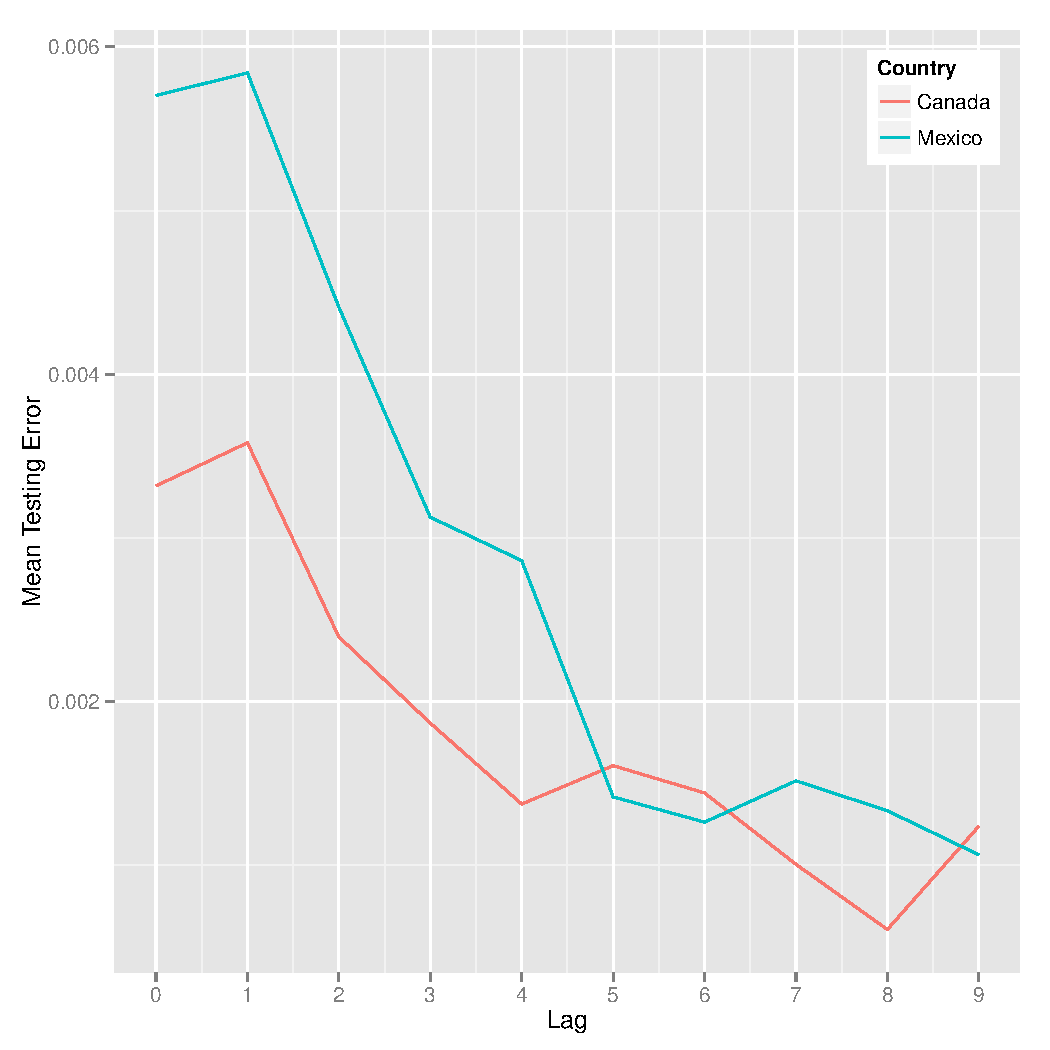
\includegraphics[scale=0.45]{lag1.pdf}
\label{fig:lag1}
\end{figure}

\begin{figure}
\centering
\caption{Model Performance for Various Lags}
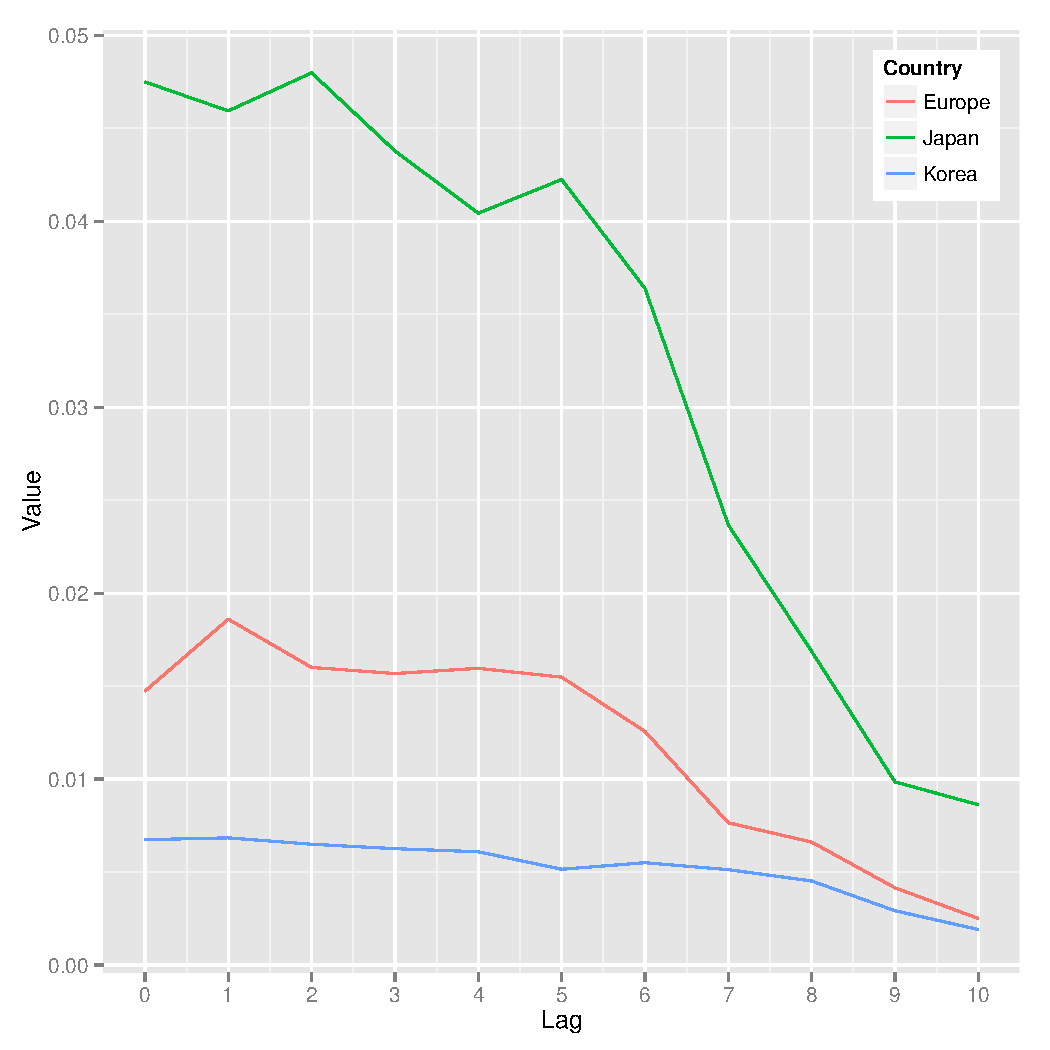
\includegraphics[scale=0.45]{lag2.pdf}
\label{fig:lag2}
\end{figure}

%\begin{figure}
%\centering
%\caption{Model Performance for Various Lags}
%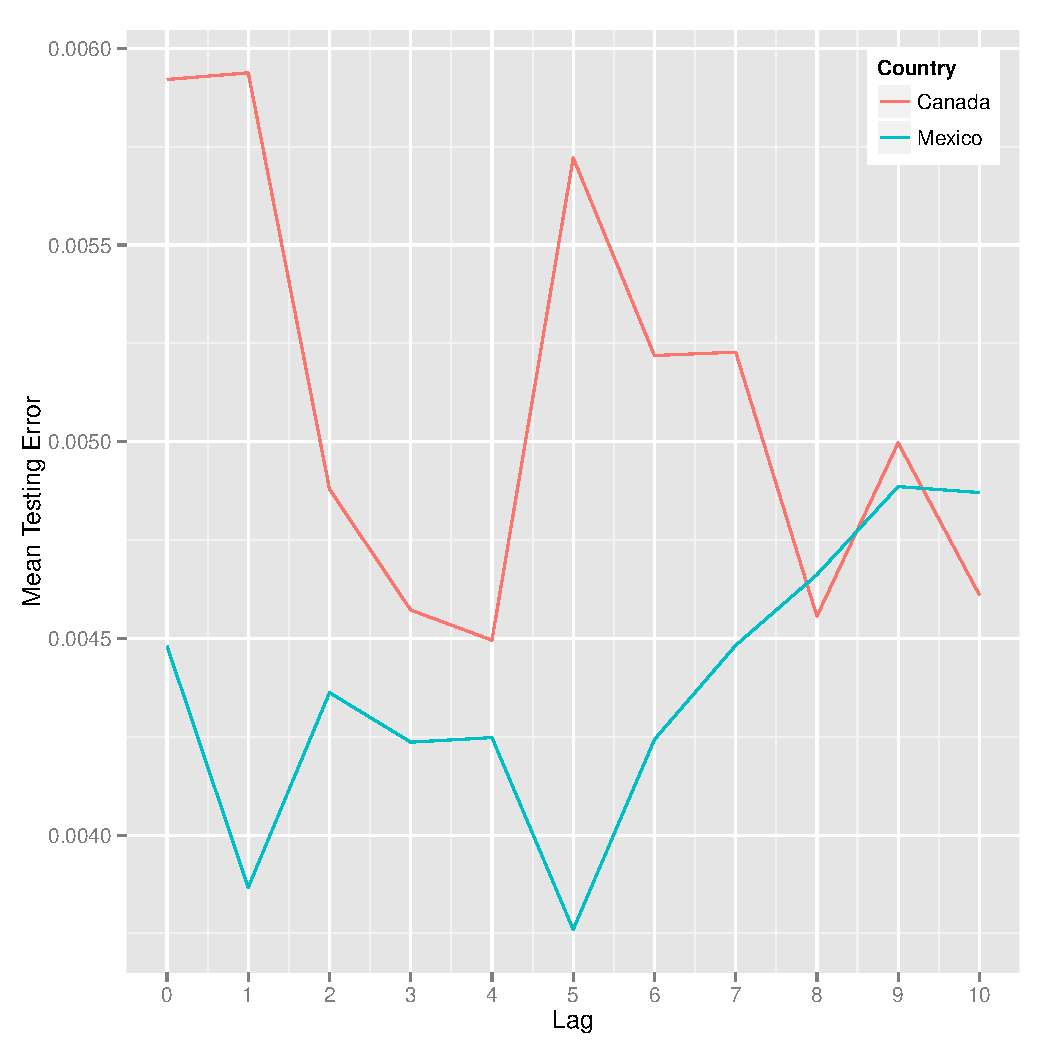
\includegraphics[scale=0.45]{ForestLag1.pdf}
%\label{fig:ForestLag1}
%\end{figure}

%\begin{figure}
%\centering
%\caption{Model Performance for Various Lags}
%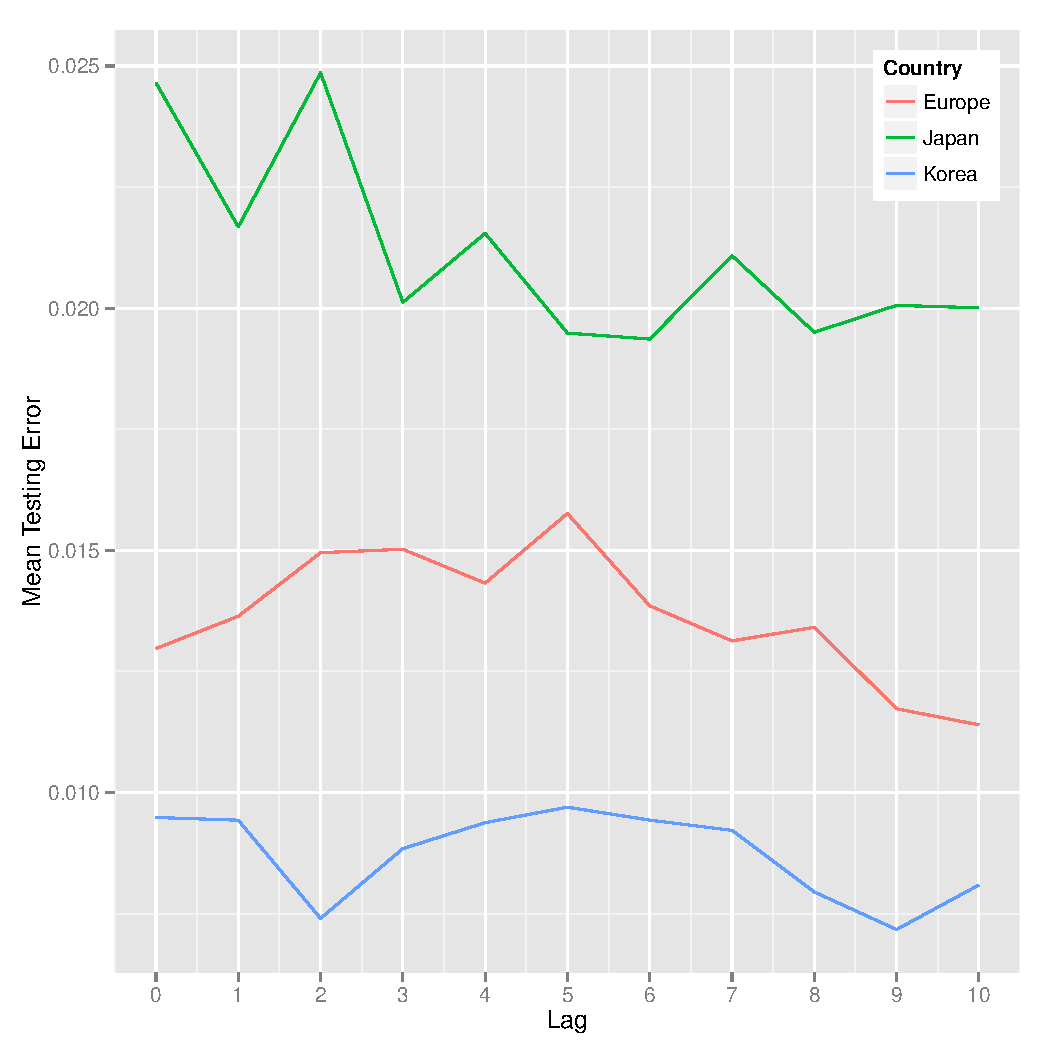
\includegraphics[scale=0.45]{ForestLag2.pdf}
%\label{fig:ForestLag2}
%\end{figure}

We determined an appropriate lag by comparing the performance of a standard linear regression model across a variety of lags. In order to find the simplest model specification that provides accurate predictions, we chose the lag by looking for the point at which including an additional month of lag stops improving the performance of the model. To do this, we plotted the mean training error of the model as a function of the lag for each country. These plots appear in Figures ~\ref{fig:lag1} and ~\ref{fig:lag2}. %, ~\ref{fig:ForestLag1}, and ~\ref{fig:ForestLag2}. 

\par{} The appropriate lag varies by country for linear models. Noticeable improvements in the performance of the model cease after month four for Canada and month five for Mexico. The results justify including lagged variables out to nine months for Europe, Japan and Korea. In the case of Korea, the decision to include a lengthy lag on the variables is less clear cut, since the model also performs well with shorter lags. However, the mean testing error decreases by a factor of two after the ninth month is included, making the increased complexity of the model worthwhile.
\par{} Including lagged variables results in a large number of possible predictors for each model. Using the lags chosen above, there are 42 possible predictors for the Canada model, 49 for the Mexico model and 77 each for the Europe, Japan and Korea models. The variables used to predict the percent change in the exchange rate were chosen by forward stepwise variable selection, as described in the methods section. These variables and their lags appear in the appendix. Of note is that at least 9 of the 12 variables in the data set appear in each of the final models chosen by forward stepwise variable selection. In addition, each variable appeared in at least two of the models. This indicates that each variable is useful as a predictor of exchange rates, as economic theory suggests they should be.

\subsection{Method Comparison}

\begin{figure}
\centering
\caption{Mean Testing Error}
\begin{tabular}{l l l l l l}
Country	& Standard 	& Ridge 		& Lasso 		& PCR 		& Naive \\
Canada 	& 0.00137 	& 0.00139 	& 0.00140 	& 0.00153 	& 0.0063 \\
Europe	& 0.00415 	& 0.00438 	& 0.00434 	& 0.00386 	& 0.0115 \\
Mexico	& 0.00141 	& 0.00149 	& 0.00173 	& 0.00148  & 0.0114 \\
Japan	& 0.00984 	& 0.00984 	& 0.00962 	& 0.00960  & 0.0205 \\
Korea	& 0.00291 	& 0.00293 	& 0.00310 	& 0.00251 	& 0.0128 \\
\end{tabular}
\label{tab:comparison}
\end{figure}




The mean testing errors for the 100 random partitions of the data set appear in Figure~\ref{tab:comparison} for each country and linear estimation technique. The naive estimate is a random walk and always predicts no change in the exchange rate after one year. This estimate is used as a baseline for assessing the usefulness of the statistical models. Each of the estimation techniques outperformed the random walk. The improvement in mean testing error ranged from a factor of two for Japan to a factor of ten for Mexico. For each method, we tested the hypothesis that the mean testing error for the model is less than the mean testing error for the random walk using a pairwise two sample t-test. The results were statistically significant at well below the 1\% significance level in each case.
\par{} A noteworthy observation from the results table is that the mean testing error does not change much when different linear techniques are used to estimate the model. For each country, we tested the hypothesis that the mean testing errors for the ridge, LASSO and principal component regressions were different than the mean testing error for the standard linear model. Although the differences were statistically significant in some cases, the magnitude of the difference was very small in every case. In practice, this means that each of the models will produce similar results. Since using more sophisticated regression techniques does not improve the performance of the model, these results support estimating the model using a standard linear regression. In fact, the primary difficulty in producing a good model is not selecting the best estimation technique, but rather choosing the correct predictors. While the results were robust to the estimation technique, they were highly sensitive to the variables included in the model, particularly the months of lag. This makes preliminary work to determine a close to optimal lag vital to producing a useful model.

\begin{figure}
\centering
\caption{Mean Testing Error - Tree Based Methods}
\begin{tabular}{l l l l l}
Country	& Full Tree & Pruned    & Forest    & Naive \\
Canada 	& 0.00739 	& 0.00734 	& 0.00450 	& 0.0063 \\
Europe	& 0.01856 	& 0.01865 	& 0.01173	& 0.0115 \\
Mexico	& 0.00707 	& 0.00706 	& 0.00376   & 0.0114 \\
Japan	& 0.03172 	& 0.03112 	& 0.02006   & 0.0205 \\
Korea	& 0.01053 	& 0.01001 	& 0.00717	& 0.0128 \\
\end{tabular}
\label{tab:treecomparison}
\end{figure} 

\par{} In contrast to linear models, changing the lag did not decrease the testing error for the tree based models. The tree based models also performed slightly worse than the linear models. The final tree based models were estimated using the same variables as the final linear models. However, none of the tree based methods were very sensitive to the variables included in the model. Figure~\ref{tab:treecomparison} shows the results for each country and method. The random forest model gave the best result of the  tree based methods. This model outperformed the random walk for all trading partners except for Europe. For Japan, it only outperformed a random walk by a small margin. In all cases, random forests performed worse than linear methods by up to an order of magnitude. The other tree based methods performed worse than the random walk for most countries. Full tree models and pruned tree models only out performed a random walk for Mexico and Korea, but the margins were not statistically significant. In general, tree based methods proved less effective than linear models for predicting exchange rates. It is possible that the reason tree based methods do not perform well is because, even though there are a large number of possible predictors, they can be approximated by a small number of principal components. This makes it difficult for decision trees to partition the data set in a way that is useful for prediction. In general, empirical evidence shows that tree based methods are not competitive with linear methods in low dimensional feature spaces. The results in this paper are consistent with these observations.


\section{Findings}

This paper shows that it is possible to predict the percent change in the exchange rate after one year, using macroeconomic indicators as predictors. In this paper, we considered both linear models and tree based methods. Each of the linear models outperformed a random walk, which is used as a baseline for assessing the usefulness of exchange rate models. This result held for each country we considered. In addition, the results show that the predictions for do not change substantially when different linear estimation techniques are used. Instead, they are sensitive the which variables are used as input. This makes choosing an appropriate lag and performing proper variable selection a vital step in producing a good model. In contrast, tree based methods were not sensitive to changes in the input variables. Despite being less sensitive, they performed considerably worse than linear models, although they did outperform a random walk. In all the evidence suggests that linear methods that carefully account for the nature of the time series are the best option for predicting exchange rates.

Linear models perform well enough that they could have a significant impact on business decisions. Writing the exchange rate values implied by the model into medium term contracts instead of the current exchange could substantially reduce the risk of conducting business internationally. A Mexican manufacturer might expect to save roughly \$70,000 on a \$1,000,000 contract with an American buyer by avoiding adverse currency movements. Clearly, accurately predicting exchange rates can help business leaders make more informed decisions.

Future work on this problem might consider different countries or variables. Since the countries chosen for this paper are major US trading partners, their exchange rates are closely related to US economic indicators. It may be more difficult to model exchange rates for large countries that trade proportionally less with the US, such as India. In addition, new variables could be considered in future work. In particular, exchange rates are sensitive to the perception of market participants. While the impact of this is more significant in the short term, it may be interesting to consider whether it persists for longer time intervals. In all, while we achieved our primary goals in this paper, predicting exchange rates is complex and ripe for continued research.  


     
% hangref environment
\newenvironment{hangref}{\begin{list}{}{\setlength{\itemsep}{0pt}
\setlength{\parsep}{0pt}\setlength{\rightmargin}{0pt}
\setlength{\leftmargin}{+\parindent}
\setlength{\itemindent}{-\parindent}}}{\end{list}}
\section*{REFERENCES}
\begin{hangref}

\item Frankel, J., and A. Rose. 1996.
``A panel project on purchasing power parity: mean reversion within and between countries.''
{\it Journal of International Economics} 40: 209-224.

\item Hsieh, D. 1989
``Testing for Nonlinear Dependence in Daily Foreign Exchange Rate Changes.''
{\it Journal of Business} 62: 329-368.

\item Krugman, P., M. Obstfeld and M.Melitz.  2014.
{\it International Economics: Theory and Policy}. 10th ed.
Upper Saddle River, New Jersey: Pearson Education.

\item Juselius, K. 1995.
``Do purchasing power parity and uncovered interest rate parity hold in the long run? An example of likelihood inference in a multivariate time-series model.''.
{\it Journal of Econometrics} 69: 211-240.

\item Lyons, K.R. and M.D.D. Evans. 2002
``Order Flow and Exchange Rate Dynamics.''
{\it Journal of Political Economy} 110: 170-180

\item Meese, R., and K. Rogoff. 1983.
``Empirical exchange rate models of the seventies: Do they fit out of sample?.'' 
{\it Journal of International Economics} 14: 3-24.

\item Meese, R.A. and A.K. Rose. 1990
``Nonlinear, Nonparametric, Nonessential Exchange Rate Estimation.''
{\it The American Economic Review} 80: 192-196 

\item Obstfeld, M., and A. Taylor. 2003.
``Globalization and capital markets.'' 
{\it Globalization in historical perspective}
University of Chicago Press: 121-188.

\item Panda, C. and V. Narasimhan 2007
``Forecasting exchange rate better with artificial neural network.''
{\it Journal of Policy Modeling} 29: 227-236

\item Wooldridge, J. 2009.
{\it Introductory Econometrics}. 4th Ed.
Mason, Ohio: South-Western Cengage Learning.

\end{hangref}

\clearpage


%\begin{figure}
%\centering
%\caption{Variables and Lags -- Canada}
%\begin{tabular}{l l}
%Variable 					& Lags  \\
%Exchange Rate 				& 0,2,4		\\
%Domestic Bond Yield			& 1,2,3,4		\\
%Foreign Bond Yield			& 0,1,3,4		\\
%Domestic Interest Rate		& 0,3,4		\\
%Foreign Interest Rate		& 0,2		\\
%Domestic Inflation Rate		& 2,4		\\
%Foreign Inflation Rate		& 0,3,4		\\
%Domestic GDP Growth			& 0		\\
%Foreign GDP Growth			& 0		\\
%Domestic Balance of Trade	& 0		\\
%Foreign Balance of Trade		& None		\\
%Foreign Exchange Reserves	& 0		\\
%\end{tabular}
%\label{tab:canada_vars}
%\end{figure}

%\begin{figure}
%\centering
%\caption{Variables and Lags -- Europe}
%\begin{tabular}{l l}
%Variable 					& Lags  \\
%Exchange Rate 				& 0,9		\\
%Domestic Bond Yield			& 0,5,7		\\
%Foreign Bond Yield			& 1,4,9		\\
%Domestic Interest Rate		& 3,	6,8,9	\\
%Foreign Interest Rate		& 5,6		\\
%Domestic Inflation Rate		& 0,	6		\\
%Foreign Inflation Rate		& 4,5		\\
%Domestic GDP Growth			& 0	\\
%Foreign GDP Growth			& 0		\\
%Domestic Balance of Trade	& 0	\\
%Foreign Balance of Trade		& 0	\\
%Foreign Exchange Reserves	& None		\\
%\end{tabular}
%\label{tab:europe_vars}
%\end{figure}

%\begin{figure}
%\centering
%\caption{Variables and Lags -- Mexico}
%\begin{tabular}{l l}
%Variable 					& Lags  \\
%Exchange Rate 				& 0,2		\\
%Domestic Bond Yield			& 5		\\
%Foreign Bond Yield			& 3,4	\\
%Domestic Interest Rate		& 0,1,5	\\
%Foreign Interest Rate		& 3,5	\\
%Domestic Inflation Rate		& 0,3,5	\\
%Foreign Inflation Rate		& 0,2		\\
%Domestic GDP Growth			& 0		\\
%Foreign GDP Growth			& 0		\\
%Domestic Balance of Trade	& None	\\
%Foreign Balance of Trade		& None	\\
%Foreign Exchange Reserves	& None		\\
%\end{tabular}
%\label{tab:mexico_vars}
%\end{figure}

%\begin{figure}
%\centering
%\caption{Variables and Lags -- Japan}
%\begin{tabular}{l l}
%Variable 					& Lags  \\
%Exchange Rate 				& 0,4,8,9		\\
%Domestic Bond Yield			& 0,4	\\
%Foreign Bond Yield			& None	\\
%Domestic Interest Rate		& 3,6,9	\\
%Foreign Interest Rate		& 2,7,9	\\
%Domestic Inflation Rate		& 0	\\
%Foreign Inflation Rate		& 0,8	\\
%Domestic GDP Growth			& None	\\
%Foreign GDP Growth			& 0		\\
%Domestic Balance of Trade	& 0	\\
%Foreign Balance of Trade		& 0	\\
%Foreign Exchange Reserves	& 0	\\
%\end{tabular}
%\label{tab:japan_vars}
%\end{figure}

%\begin{figure}
%\centering
%\caption{Variables and Lags -- Korea}
%\begin{tabular}{l l}
%Variable 					& Lags  \\
%Exchange Rate 				& 0,6,9		\\
%Domestic Bond Yield			& 0,5	\\
%Foreign Bond Yield			& 8	\\
%Domestic Interest Rate		& 2,6,9	\\
%Foreign Interest Rate		& 7,9	\\
%Domestic Inflation Rate		& 1,3,5,6,9	\\
%Foreign Inflation Rate		& 0,9	\\
%Domestic GDP Growth			& None	\\
%Foreign GDP Growth			& None		\\
%Domestic Balance of Trade	& 0	\\
%Foreign Balance of Trade		& None	\\
%Foreign Exchange Reserves	& 0	\\
%\end{tabular}
%\label{tab:korea_vars}
%\end{figure}







\end{document}
